\documentclass[12pt]{article}
\usepackage{graphicx,psfrag,amsfonts,float,mathbbol,xcolor,cleveref}
\usepackage{arydshln}
\usepackage{amsmath}
\usepackage{tikz}
\usepackage[mathscr]{euscript}
\usepackage{enumitem}
\usepackage{accents}
\usepackage{lscape}
\usepackage{framed}
\usepackage{subcaption}
\usepackage{natbib}
\usepackage{mathtools}
\usepackage{IEEEtrantools}
\usepackage{times}

\usepackage{filecontents}
\usepackage{subfiles}
\usepackage{cite}
\usepackage{rotating}
\usepackage{arydshln}
\usepackage{amsthm}
\usepackage[letterpaper, left=1in, top=1in, right=1in, bottom=1in,nohead,includefoot, verbose, ignoremp]{geometry}
\usepackage{booktabs}
\newcommand{\ra}[1]{\renewcommand{\arraystretch}{#1}}
\newcommand\numberthis{\addtocounter{equation}{1}\tag{\theequation}}
\newcommand*\needsparaphrased{\color{red}}
\newcommand*\needscited{\color{orange}}
\newcommand*\needsproof{\color{blue}}
\newcommand*\outlineskeleton{\color{green}}
\newcommand{\PP}{\mathcal{P}}
\newcommand{\hilbert}{\mathcal{H}}
\newcommand{\hilbertl}{\mathcal{H}_{\langle l \rangle}}
\newcommand{\hilbertm}{\mathcal{H}_{\langle m \rangle}}
\newcommand{\hilbertlnull}{\mathcal{H}_{0\langle l \rangle}}
\newcommand{\hilbertmnull}{\mathcal{H}_{0\langle m \rangle}}
\newcommand{\hilbertlpen}{\mathcal{H}_{1\langle l \rangle}}
\newcommand{\hilbertmpen}{\mathcal{H}_{1\langle m \rangle}}

\newcommand{\bfeps}{\mbox{\boldmath $\epsilon$}}
\newcommand{\bfgamma}{\mbox{\boldmath $\gamma$}}
\newcommand{\bflam}{\mbox{\boldmath $\lambda$}}
\newcommand{\bfphi}{\mbox{\boldmath $\phi$}}
\newcommand{\bfsigma}{\mbox{\boldmath $\sigma$}}
\newcommand{\bfbeta}{\mbox{\boldmath $\beta$}}
\newcommand{\bfalpha}{\mbox{\boldmath $\alpha$}}
\newcommand{\bfe}{\mbox{\boldmath $e$}}
\newcommand{\bff}{\mbox{\boldmath $f$}}
\newcommand{\bfone}{\mbox{\boldmath $1$}}
\newcommand{\bft}{\mbox{\boldmath $t$}}
\newcommand{\bfo}{\mbox{\boldmath $0$}}
\newcommand{\bfO}{\mbox{\boldmath $O$}}
\newcommand{\bfx}{\mbox{\boldmath $x$}}
\newcommand{\bfX}{\mbox{\boldmath $X$}}
\newcommand{\bfz}{\mbox{\boldmath $z$}}
\newcommand{\argmin}[1]{\underset{#1}{\operatorname{arg}\,\operatorname{min}}\;}
\DeclareMathAlphabet{\mathpzc}{OT1}{pzc}{m}{it}

\newcommand{\bfm}{\mbox{\boldmath $m}}
\newcommand{\bfy}{\mbox{\boldmath $y$}}
\newcommand{\bfa}{\mbox{\boldmath $a$}}
\newcommand{\bfb}{\mbox{\boldmath $b$}}
\newcommand{\bfY}{\mbox{\boldmath $Y$}}
\newcommand{\bfS}{\mbox{\boldmath $S$}}
\newcommand{\bfZ}{\mbox{\boldmath $Z$}}
\newcommand{\cardT}{\vert \mathcal{T} \vert}
%\newenvironment{theorem}[1][Theorem]{\begin{trivlist}
%\item[\hskip \labelsep {\bfseries #1}]}{\end{trivlist}}
%\newenvironment{corollary}[1][Corollary]{\begin{trivlist}
%\item[\hskip \labelsep {\bfseries #1}]}{\end{trivlist}}
%\newenvironment{proposition}[1][Proposition]{\begin{trivlist}
%\item[\hskip \labelsep {\bfseries #1}]}{\end{trivlist}}
%\newenvironment{definition}[1][Definition]{\begin{trivlist}
%\item[\hskip \labelsep {\bfseries #1}]}{\end{trivlist}}

\newtheorem{theorem}{Theorem}[section]
\newtheorem{lemma}[theorem]{Lemma}
\newtheorem{proposition}[theorem]{Proposition}
\newtheorem{corollary}[theorem]{Corollary}

\theoremstyle{definition}
\newtheorem{definition}{Definition}[section]
\newtheorem{example}{Example}[section]
\def\bL{\mathbf{L}}

\begingroup\lccode`~=`_
\lowercase{\endgroup\def~}#1{_{\scriptscriptstyle#1}}
\AtBeginDocument{\mathcode`_="8000 \catcode`_=12 }

\makeatletter
\renewcommand{\theenumi}{\Roman{enumi}}
\renewcommand{\labelenumi}{\theenumi.}
\renewcommand{\theenumii}{\Alph{enumii}}
\renewcommand{\labelenumii}{\theenumii.}
\renewcommand{\p@enumii}{\theenumi.}
\makeatother

\begin{document}

%\nocite{*}
\def\bL{\mathbf{L}}
%\usepackage{mathtime}

%%UNCOMMENT following line if you have package


\title{ Nonparametric Covariance Estimation for Longitudinal Data via Penalized Tensor Product Splines}

\author{Tayler A. Blake\thanks{The Ohio State University, 1958 Neil Avenue, Columbus, OH 43201} \and  Yoonkyung Lee\thanks{The Ohio State University, 1958 Neil Avenue, Columbus, OH 43201}}

\bibliographystyle{plainnat}
\maketitle

\section{Performance assessment via simulation study}

%
%To gauge the utility of our method, we compare the performance of the estimator based on complete data to that of  three alternative estimators. 
%
%A complete dataset is one in which all subjects share a common set of evenly-spaced observation times $t_1, \dots, t_M$, and there are no observations missing for any patient. To examine the robustness of our method to sparsity in the data, we also compare our performance in the ideal sampling case to the performance of the estimator based on incomplete data by subsampling observations and treating the remaining unused observations as missing data. 

To understand the strengths and weaknesses of our method, in the first portion of our simulation study, we examine performance for five underlying covariance structures across varying numbers of subjects, $N$, and within-subject sample sizes, $M$. In the first portion of the study, we simulate data so that all subjects share a common set of $M$ regularly-spaced observation times so as to permit performance comparison with three alternative estimators based on the sample covariance matrix, which cannot accommodate irregularly spaced observations.  In the second portion of the study, our primary concern is studying the stability of our estimator as the irregularity in the observed time points across subjects increases. For fixed $N$, we observe performance when the data are generated from the same underlying covariance structures for varying within-subject sample sizes $M$ and varying levels of data sparsity by subsampling observations from the complete dataset. 

\bigskip

We study estimator performance for five covariance structures, which were chosen to exhibit varying degrees of structural complexity. At one end of the spectrum, we consider covariance corresponding to mutual independence. It is both the simplest and sparsest structure, having constant zero-valued varying coefficient function, and constant innovation variance function. To examine how well our estimator selects models belonging to the null space of the cubic smoothing spline penalty functional, we consider a class of covariance structures defined by the GARPs, which are the evaluation of a linear function of $t$, and the IVs, which are constant over the time domain. We induce three degrees of sparisty in the Cholesky factor by truncating its entries to zero at three values of $l = t - s \in \left[0,1\right]$. This is equivalent to banding the inverse covariance matrices at the same values of $l$; see \citet{bickel2008regularized}. We also consider the compound symmetry model to assess how well our method can identify a commonly utilized parametric model for longitudinal data. While the structure is of the overall covariance matrix is parsimonious in that it can be represented with few coefficients, the varying coefficient function and innovation variance function of the corresponding Cholesky decomposition are nonlinear in $t$.  Given covariance matrix $\Sigma$, risk estimates are obtained from$N_{sim} = 100$ samples from an $M$-dimensional multivariate Normal distribution with mean zero and the same covariance. 

\section{Alternative estimators for performance benchmarking}

For the complete data case with common observation times across all subjects, we consider three additional covariance estimators for comparison: the sample covariance matrix $S$, the soft thresholding estimator of \citet{rothman2009generalized},  $S^\lambda$, and the tapering estimator of \citet{cai2010optimal}, $S^\omega$. See Chapter 2, Section~\ref{section:element-wise-shrinkage-estimators} for additional discussion of these estimators and those belonging to similar classes. \citet{rothman2009generalized} presented a class of generalized thresholding estimators, including the soft-thresholding estimator given by

\[
S^{\lambda}=   \begin{bmatrix} \mbox{sign}\left(s_{ij}\right) \left(s_{ij} - \lambda\right)_+ \end{bmatrix},
\]
\noindent 
where $\sigma^*_{ij}$ denotes the $i$-$j^{th}$ entry of the sample covariance matrix, and $\lambda$ is a penalty parameter controlling the amount of shrinkage applied to the empirical estimator. \citet{cai2010optimal} derived optimal rates of convergence under the operator norm for the tapering estimator:
\[
S^{\omega} =  \begin{bmatrix} \omega_{ij}^k s_{ij} \end{bmatrix},
\]
\noindent
where the $\omega_{ij}^k$ are given by 
\begin{equation*}
\omega^k_{ij} = k_h^{-1} \left[ \left( k - \vert i-j\vert\right)_+ - \left(k_h - \vert i-j\vert\right)_+ \right],
\end{equation*}
\noindent
The weights $\omega^k_{ij}$ are indexed with superscript to indicate that they  are controlled by a tuning parameter, $k$,  which can take integer values between 0 and $M$, the dimension of the covariance matrix.  Without loss of generality,  we assume that $k_h = k/2$ is even. The weights may be rewritten as
\begin{align*}
\omega_{ij} = \left\{\begin{array}{ll} 1, & \vert \vert i -j \vert \vert \le k_h \\
                             2 - \frac{i - j}{k_h}, & k_h < \vert \vert i -j \vert \vert \le k, \\
                             0, & \mbox{otherwise}  \end{array} \right.
\end{align*}
\noindent
This expression of the weights makes it clear how the selection of $k$ controls the amount of shrinkage applied to different elements of the sample covariance matrix. The estimator applies no shrinkage to elements of $S$ belonging to the subdiagonals closest to the main diagonal. As one moves away from the main diagonal, shrinkage increases. A shrinkage factor of $2 - \frac{i - j}{k_h}$ is applied to elements belonging to subdiagonals $k_h,\dots,k-1,k$, and elements further than $k$ subdiagonals from the main diagonal are shrunk to zero.   

\section{Loss functions and corresponding risk measures}

To assess performance of estimator $\hat{\Sigma}$, we consider two commonly used loss functions:
\begin{equation} \label{eq:quad-loss}
\Delta_1\left(\Sigma,\hat{\Sigma} \right) = tr\left( \Sigma^{-1} \hat{\Sigma} \right) - log \vert \Sigma^{-1} \hat{\Sigma} \vert - M,
\end{equation}
\noindent
\begin{equation} \label{eq:entropy-loss}
\Delta_2\left(\Sigma,\hat{\Sigma}\right) = tr\left(\left( \Sigma^{-1} \hat{\Sigma} - \mathrm{I}\right)^2 \right)
\end{equation}
\noindent
where $\Sigma$ is the true covariance matrix and $\hat{\Sigma}$ is an $M \times M$ positive definite matrix. Each of these loss functions is $0$ when $\hat{\Sigma} = \Sigma$ and is positive when $\hat{\Sigma} \ne \Sigma$. Both measures of loss are scale invariant. If we let random vector $Y$ have covariance matrix $\Sigma$, and define the transformation $Z$ as

\[
Z = CY. 
\]
\noindent
for some $M \times M$ matrix $C$,  then $Z$ has covariance matrix $\Sigma_z = C \Sigma C'$. Given an estimator $\hat{\Sigma}$ of $\Sigma$, one immediately obtains an estimator for $\Sigma_z$, $\hat{\Sigma}_z = C \hat{\Sigma} C'$. If $C$ is invertible, then the loss functions $\Delta_1$ and $\Delta_2$ satisfy
\[
\Delta_i\left(\Sigma,\hat{\Sigma}\right) = \Delta_i\left(C \Sigma C', C \hat{\Sigma}C' \right). 
\]
\noindent
The first loss $\Delta_1$ is commonly referred to as the entropy loss; it gives the Kullback-Leibler divergence of two multivariate Normal densities with the same mean corresponding to the two covariance matrices. The second loss $\Delta_2$, or the quadratic loss, measures the discrepancy between $\left(\Sigma^{-1} \hat{\Sigma}\right)$ and the identity matrix with the squared Frobenius norm. The Frobenius norm of a symmetric matrix $A$ is given by 

\[
\vert \vert A \vert \vert^2 = \mbox{tr}\left(A A'\right).
\]
\noindent
The quadratic loss consequently penalizes overestimates more than underestimates, so ``smaller'' estimates are favored more under $\Delta_2$ than $\Delta_1$. For example, among the class of estimators comprised of scalar multiples $cS$ of the sample covariance matrix, \citet{haff1980empirical} established that $S$ is optimal under $\Delta_2$, while the smaller estimator $\frac{nS}{n+p+1}$ is optimal under $\Delta_1$. 

\bigskip

Given $\Sigma$, the corresponding values of the risk functions are obtained by taking expectations:

\begin{equation*}
R_i \left(\Sigma,\hat{\Sigma}\right) = E_\Sigma\left[\Delta_i\left(\Sigma,\hat{\Sigma}\right)\right], \quad i = 1,2.
\end{equation*}
\noindent
We prefer one estimator $\hat{\Sigma}_1$ to another $\hat{\Sigma}_2$ if it has smaller risk.  Given $\Sigma$, we estimate the risk of an estimator via Monte Carlo approximation. 

\section{Discussion}

For each of the general covariance structures outlined in the previous simulation study description, data were simulated according to multivariate normal distributions with the following covariance matrices: 
\begin{enumerate} 
\item\label{item:cov-type-1} Mutual independence: $\Sigma = \mathrm{I}$, where 
\begin{align*}
\phi\left(t,s\right) &= 0, \quad 0 \le s < t \le 1,\\ 
\sigma^2\left(t\right) &= 1, \quad 0 \le t \le 1.
\end{align*}
\item \label{item:cov-type-2} Linear varying coefficient model with constant innovation variance: $\Sigma^{-1} = T' D^{-1} T$, where 
\begin{align*}
\phi\left(t,s\right) &= t - \frac{1}{2},  \quad 0 \le t \le 1, \\
\sigma^2\left(t\right) &= 0.1^2,  \quad 0 \le t \le 1.
\end{align*}
{\needsparaphrased{TODO: How do we describe the structures for models II-V in terms of continuous $t\in\left[0,1\right]$? }}
\item \label{item:cov-type-3} $k_{1/2}$-banded linear varying coefficient model with constant innovation variance: $\Sigma^{-1} = T' D^{-1} T$, where
\begin{align*}
\phi\left(t,s\right) &= \left\{\begin{array}{ll} t - \frac{1}{2}, & t - s \le 0.5\\ 
0, & t - s > 0.5\end{array}\right.,\\
\sigma^2\left(t\right) &= 0.1^2, \quad 0 \le t \le 1.
\end{align*}
\item \label{item:cov-type-4} $1$-banded linear varying coefficient model with constant innovation variance: $\Sigma^{-1} = T' D^{-1} T$ where 
\begin{align*}
\phi\left(t,s\right) &= \left\{\begin{array}{ll} t - \frac{1}{2}, & t - s \le \frac{1}{M}\\ 0, & t - s > \frac{1}{M}\end{array}\right.,\\
\sigma^2\left(t\right) &= 0.1^2, \quad 0 \le t \le 1.
\end{align*}
\item \label{item:cov-type-5} The compound symmetry model: $\Sigma = \sigma^2\left(\rho \mathrm{J} + \left(1-\rho\right)\mathrm{I}\right),\; \rho=0.7,\;\sigma^2=1$. 
\begin{align*}
\phi_{ts} &= -\frac{\rho}{1 + \left(t-1\right)\rho}, \quad t = 2, \dots, M,\;\; s = 1, \dots, t-1\\
\sigma_t^2 &= \left\{\begin{array}{ll} 1, & t = 1\\ 1 -\frac{\left(t-1\right)\rho^2}{1 + \left(t-1\right)\rho}, & t = 2, \dots, M \end{array}\right.
\end{align*}
\end{enumerate}

{\needsparaphrased{TODO: Include figures of the true Cholesky surfaces for models 2-5.}}



\begin{figure}[H] \label{fig:cov-type-2}
\begin{center}
    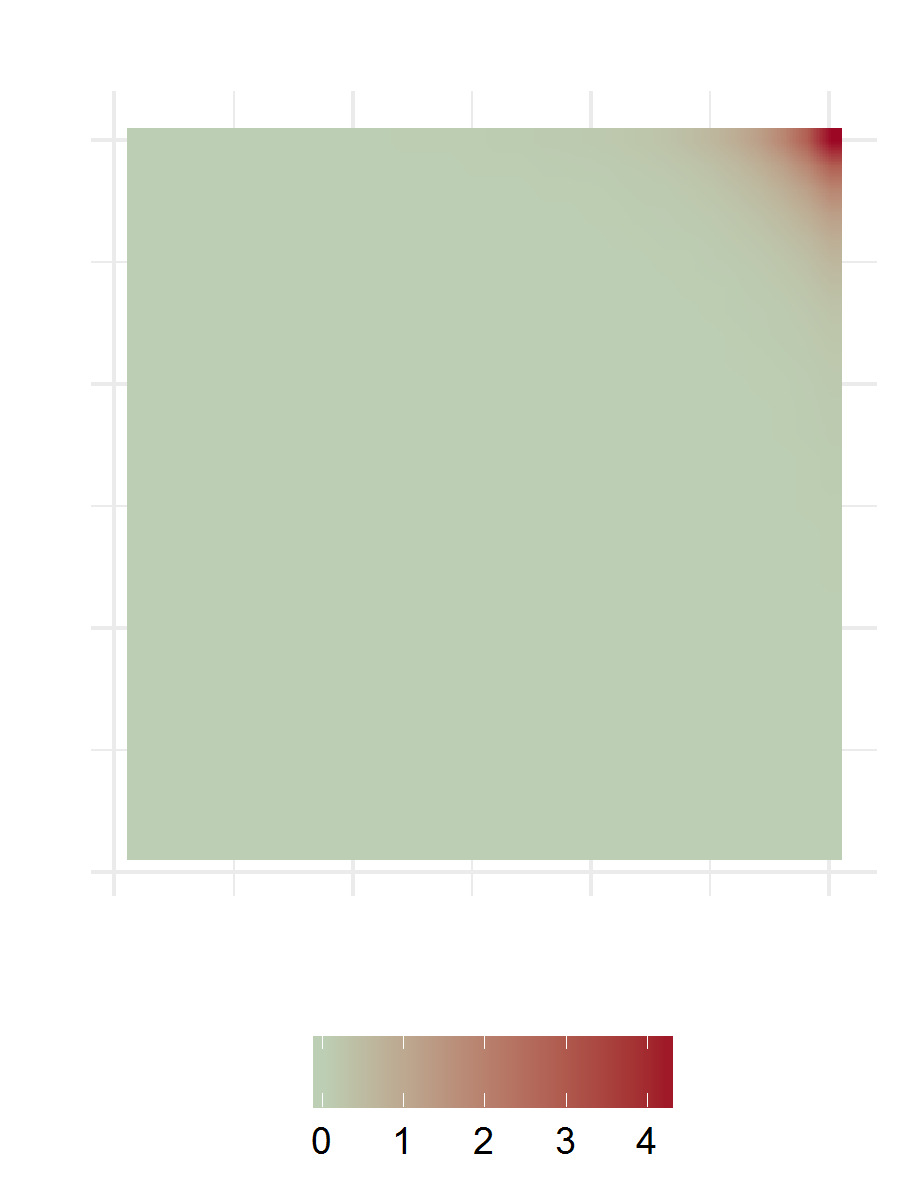
\includegraphics[width=\textwidth]{../img/chapter-4/simulation-covariance-structure-3-heat-map}
\end{center}
 \caption{covariance surface corresponding to Model~\ref{item:cov-type-2}}
 \end{figure}

\begin{figure}[H] \label{fig:cov-type-3}
\begin{center}
 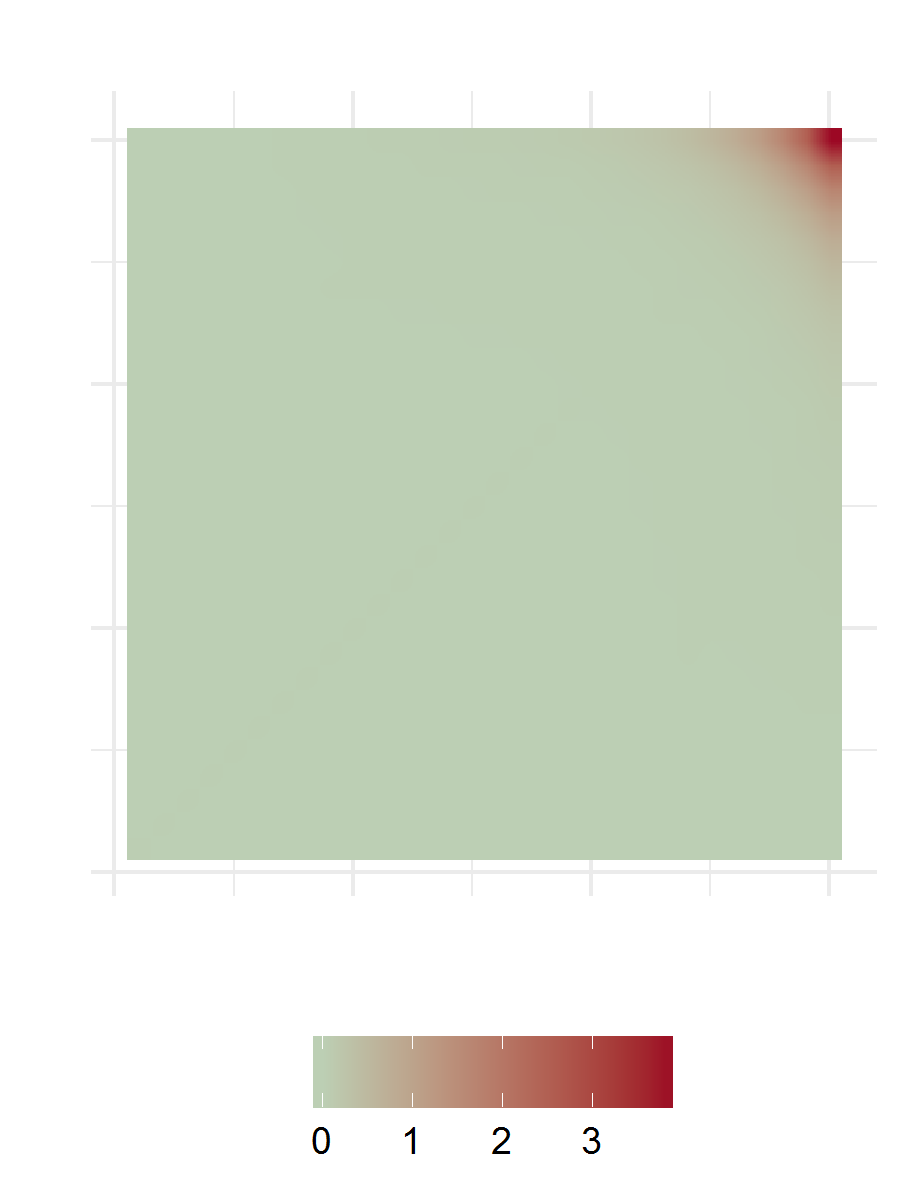
\includegraphics[width=\textwidth]{../img/chapter-4/simulation-covariance-structure-2-heat-map}
\end{center}
 \caption{covariance surface corresponding to Model~\ref{item:cov-type-3}}
\end{figure} 


\begin{figure}[H] \label{fig:cov-type-4}
\begin{center}
 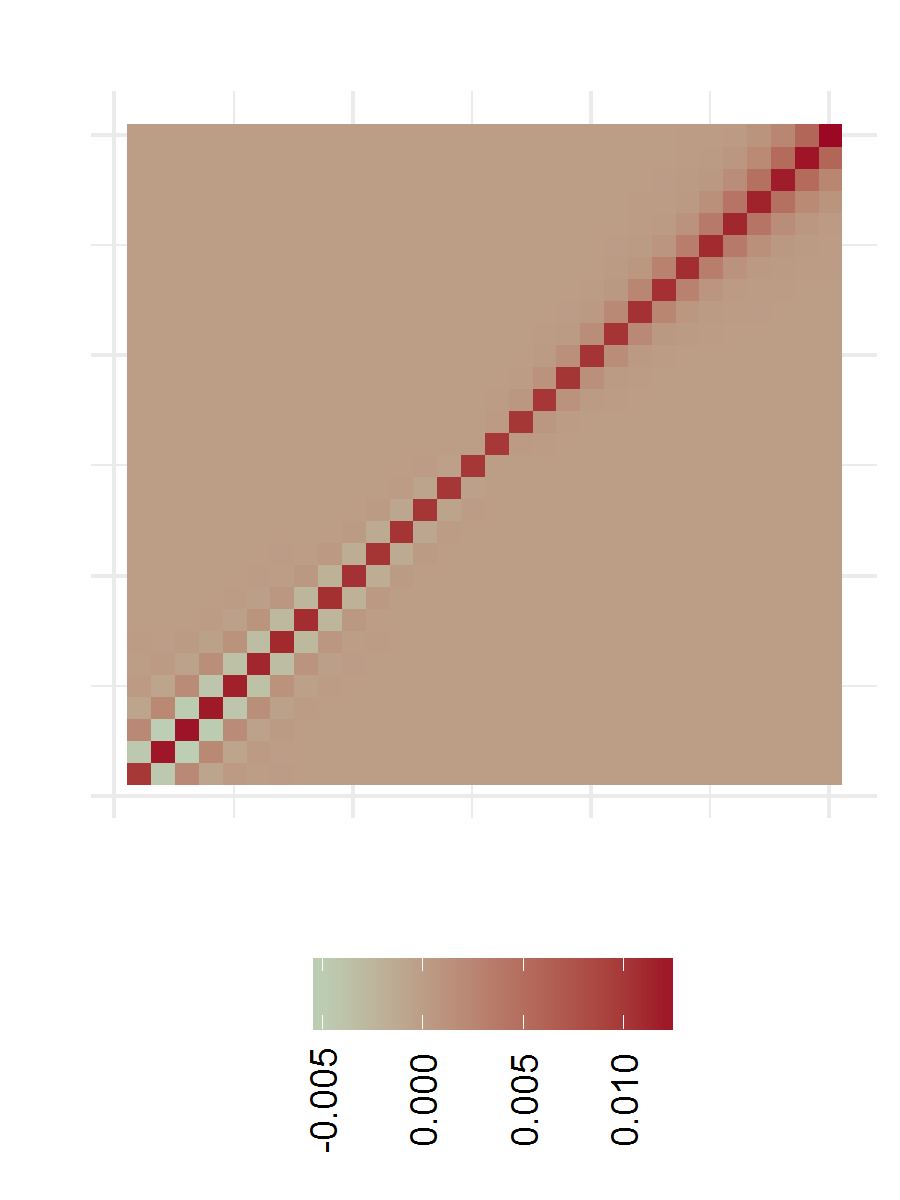
\includegraphics[width=\textwidth]{../img/chapter-4/simulation-covariance-structure-4-heat-map}
\end{center}
 \caption{covariance surface corresponding to Model~\ref{item:cov-type-4}}
\end{figure} 


\bigskip

The results of the simulations for complete data under entropy loss are presented in tables \ref{table:simulation-1-entropy-loss-sigma-1} - \ref{table:simulation-1-entropy-loss-sigma-5}; the results for quadratic loss are similar and can be found in the Appendix, Table~\ref{table:simulation-1-quad-loss-sigma-1}-\ref{table:simulation-1-quad-loss-sigma-5}. The results for the second simulation study of performance with sparsely sampled data are given in tables \ref{table:simulation-2-sigma-1} - \ref{table:simulation-2-sigma-5}.  Standard errors of the risk estimates are left to the appendix; see Table~\ref{table:ssanova-estimator-performance-with-se-ure} and Table~\ref{table:ssanova-estimator-performance-with-se-loso}.

\bigskip


Our estimator is stable across all of the underlying covariance  structures for the differing number of sampled trajectories $N = 50, 100$, while the performance of the alternative estimators markedly improves when the subject sample size is doubled for each of the generating structures, particularly for the case of $M = 30$. Irrespective of tuning parameter selection method, our estimator is preferable to all three of the alternative estimators, except under Model IV when $N$ is large and within-subject sampling rates are moderate. Under this model, both the inverse covariance as well as the covariance matrix itself are sparse. Specifically, the inverse is banded so that $\sigma^{ij} = 0$ for $\vert i - j \vert > 1$, but the non-zero elements are quite large. Inversion results in a covariance matrix which decays quickly as distance from the main diagonal increases, which is in concordance with the assumed structure of the softthresholding estimator. 

\bigskip

The covariance matrix corresponding to Model II is highly nonstationary. It is neither sparse, nor has entries which decrease in absolute value as the time between observations increases, which is in discordance with the assumed structure of both element-wise shrinkage estimators. However, on every subdiagonal are entries which are very small. The tapering estimator performs abysmally for this structure, since for almost any choice of $k$, it will incorrectly be shrinking many entries which are large in absolute values to zero. The soft thresholding estimator assumes no implicit structure of the $M$ measurements which make up the random vector (it does not assume that $y_1,\dots, y_M$ are time-ordered.) While the covariance is nonstationary, the elements of $\Sigma$ are highly structured, but the soft-thresholding esitmator fails to exploit this structure which results in $S^\lambda$ having 0s spuriously placed. The covariance matrix under Model III has similar structure, presenting similar difficulties for both estimators. The sample covariance matrix far outperforms both of its regularized renditions almost uniformly across subject sample sizes $N$ for moderate within-subject sampling rates ($M = 20, 30$.)
 
\bigskip

Performance degradation of the estimator in the presence of missing data is highly dependent on the underlying structure of the Cholesky factor of the inverse covariance matrix. For the identity matrix and for the non-truncated linear varying coefficient GARP model, we observe little change in estimated entropy risk for within subject sample sizes $M = 10$ and $M = 20$ with downsampling as compared to the estimated risk for both sample sizes in the complete data case. Making the same comparison for the banded Cholesky factor having linear varying coefficient function truncated at $t = 0.5$, we see only slight decreases in performance for $M = 10$: an estimated entropy risk of 0.3174  with no missing data versus 0.3451 (0.3498, 0.3437) with $5\%$ ($7\%$, $9\%$) missing data. The degredation is more pointed for the moderate sample size of $M = 20$. The rate of missing observations has the greatest impact for the simulation conducted using the compound symmetric model. This is not surprising, since it corresponds to the Cholesky factor having the most complex structure. While the functions defining the Cholesky factors of Models III and IV do not belong to the null space defined by the cubic smoothing spline penalty, they are both piecewise functions with each piece itself belonging to $\mathcal{H}_0$.

\bigskip

{\needsparaphrased{Should the discussion that immediately follows be moved to after the tables containing non-appendix numerical results?}}

\bigskip

{\needsparaphrased{Should the discussion of study \# 1 be with the tablse for study 1, separate from the discussion + tables for study 2?}}

\bigskip

Review of generalized thresholding estimators, including the soft thresholding estimator is presented in in \ref{subsubsection:chapter-1-sss-1-3-4}. Recall that  $S^\lambda$ can be written as the solution to the optimization problem

\begin{equation} \label{eq:soft-thresholding-objective-function}
\mathpzc{s}_\lambda\left( z \right)  = \argmin{\sigma} \left[ \frac{1}{2} \left(\sigma - z\right)^2 + J_\lambda\left(\sigma \right)\right],
\end{equation}
\noindent
so that estimation of the covariance matrix can be accomplished by solving multiple univariate Lasso-penalized least squares problems. 
%The Frobenius is a natural measure of the accuracy of an estimator; it quantifies the sum over the unique elements of $\Sigma$ of the the first term in \ref{eq:soft-thresholding-objective-function}, 
%
%\begin{equation} \label{eq:forbenius-norm}
%\vert \vert  \hat{\Sigma}^\lambda - \Sigma \vert \vert^2 = \left(\sum_{i,j} \left(\hat{\sigma}^\lambda_{ij} - \sigma_{ij} \right)^2\right)^{1/2}
%\end{equation}
%\noindent
%If $\Sigma$ were available, one would choose the value of the tuning parameter $\lambda$ which minimizes \ref{eq:frobenius-norm}. In practice, one tries to first approximate the risk, or 
%\[
%E_\Sigma\left[\vert \vert  \hat{\Sigma}^\lambda - \Sigma \vert \vert^2 \right],
%\]
%\noindent
%and then choose the optimal value of $\lambda$.  As in regression methods, cross validation and a number of its variants have become popular choices for tuning parameter selection in covariance estimation. $K$-fold cross validation requires first splitting the data into folds $\mathcal{D}_1, \mathcal{D}_2, \dots, \mathcal{D}_K$. 

\bigskip

Under certain conditions pertaining to the ration of sample sizes of the training and validation datasets, the $K$-fold cross validation criterion is a consistent estimator of the Frobenius norm risk. It is defined 

\begin{equation} \label{eq:K-fold-matrix--cv}
\mbox{CV}_F\left(\lambda \right) = \argmin{\lambda} K^{-1} \sum_{k = 1}^K  \vert \vert\hat{\Sigma}^{\left(-k\right)} - \tilde{\Sigma}^{\left(k\right)}  \vert \vert_F^2, 
\end{equation}
\noindent
%where $\tilde{\Sigma}^{\left(k\right)}$ is the unregularized estimator based on based on $\mathcal{D}_k$, and $\hat{\Sigma}^{\left(-k\right)}$ is the regularized estimator under consideration based on the data after holding $\mathcal{D}_k$ out.  Using this approach, the size of the training data set is approximately $\left(K - 1 \right)N/K$, and the size of the validation set is approximately $N/K$ (though these quantities are only relevant when subjects have equal numbers of observations). For linear models, it has been shown that cross validation is asymptotically consistent is the ratio of the validation data set size over the training set size goes to 1. See \citet{shao1993linear}. This result motivates the reverse cross validation criterion, which is defined as follows:
%
%\begin{equation} \label{eq:K-fold-matrix-reverse-cv}
%\mbox{rCV}_F\left(\lambda \right) = \argmin{\lambda} K^{-1} \sum_{k = 1}^K  \vert \vert\hat{\Sigma}^{\left(k\right)} - \tilde{\Sigma}^{\left(-k\right)}  \vert \vert_F^2, 
%\end{equation}
%\noindent
%where $\tilde{\Sigma}^{\left(-k\right)}$ is the unregularized estimator based on based on the data after holding out $\mathcal{D}_k$, and $\hat{\Sigma}^{\left(k\right)}$ is the regularized estimator under consideration based on $\mathcal{D}_k$. 
There is little established about the optimal method for tuning parameter selection in for the class of estimators based on element-wise shrinkage of the sample covariance matrix.  However, based on the results of an extensive simulation study presented in \citet{fang2016tuning}, we use $K = 10$-fold cross validation to select the tuning parameters for both the tapering estimator $S^\omega$ and the soft thresholding estimator $S^{\lambda}$. They authors implement cross validation for a number of element-wise shrinkage estimators for covariance matrices in the \citet{CVTuningCov} R package, which was used to calculate the risk estimates for $S^{\omega}$ and $S^{\lambda}$. 

\bigskip


Element-wise shrinkage estimators of the covariance matrix, including the soft thresholding estimator, are not guaranteed to be positive definite, though \citet{rothman2009generalized} established that in the limit, soft thresholding produces a positive definite estimator with probability tending to 1.  We observed simulations runs which yielded a soft thresholding estimator that was indeed not positive definite.   In this case, the estimate has at least one eigenvalue less than or equal to zero, and the evaluation of the entropy loss \ref{eq:entropy-loss} is undefined. To enable the evaluation of the entropy loss, we coerced these estimates to the ``nearest'' positive definite estimate via application of the technique presented in \citet{cheng1998modified}.  For a symmetric matrix $A$, which is not positive definite,  a modified Cholesky algorithm produces a symmetric perturbation matrix $E$ such that $A + E$ is positive definite.

\bigskip

{\needsparaphrased{We need to decide which tables will be included in the non-appendix numerical results. In the actual dissertation, section 6 will not immediate follow section 5.}}

\bigskip

\section{Numerical results}
%%%%%%%%%%%%%%%%%%%%%%%%%%%%%%%%%%%%%%%%%%%%%%%%%%%%%%%
\subsection{Simulation study 1: complete data}

\setlength{\dashlinedash}{0.5pt}
\setlength{\dashlinegap}{1pt}
\setlength{\arrayrulewidth}{0.2pt}

%% entropy risk
\begin{table}[H] \label{table:simulation-1-entropy-loss-sigma-1}
\centering
\caption{Risk estimates and corresponding standard errors for our proposed estimator under entropy loss, $\Delta_2$ when the data are generated according to model~\ref{item:cov-type-1}.} 
\begin{tabular}{l|r|rrrrrr}
&  & \multicolumn{2}{c}{$\hat{\Sigma}_{SS}$} & $S$ & $S^\lambda$ & $S^\omega$ \\ 
&M & \mbox{LosoCV} & \mbox{URE} &  \\ 
  \hline
&    10 & 0.0684 & 	0.0678	&1.2339 & 0.4451 & 1.1760\\ 
$N = 50$ &    20 & 0.0799 & 	0.0720	&5.0827 & 1.6504 & 4.7847 \\ 
  &    30 & 0.0668 &	0.0740	 &12.5162  & 1.9975 & 11.0434 \\ 
   \hdashline
 &    10 & 0.0405 & 0.0379 & 0.5854  & 0.1783 & 0.5201 \\ 
$N = 100$ &    20 & 0.0356 &  0.0378 & 2.3038 & 0.4394 & 1.9637 \\ 
  &    30 & 0.0396 & 0.0322  &5.2641 & 0.6717 & 4.5410 \\ 
\end{tabular}
\end{table}


%-------------------------------------------------------------------------------------------------------------------------------------------

\begin{table}[H] \label{table:simulation-1-entropy-loss-sigma-2}
\centering
\caption{Risk estimates and corresponding standard errors for our proposed estimator under entropy loss, $\Delta_2$ when the data are generated according to model~\ref{item:cov-type-2}.} \begin{tabular}{l|r|rrrrrr}
&  & \multicolumn{2}{c}{$\hat{\Sigma}_{SS}$} & $S$ & $S^\lambda$ & $S^\omega$ \\ 
&M & \mbox{LosoCV} & \mbox{URE} &  \\ 
  \hline
 &    10 & 0.0647 & 0.0696	 & 1.2431 & 1.4242 & 1.1195\\ 
$N = 50$ &    20 & 0.0884 & 0.0969 & 5.0437 & 17.0220 & 13.5290\\ 
&    30 & 0.0702 & 0.0894 & 12.4559 & 39.9769 & 159.0521 \\ 
   \hdashline
&    10 & 0.0307 & 0.0302 & 0.5403& 0.7659 & 0.5609 \\ 
$N = 100 $ &    20 & 0.0357 & 0.0350  & 2.3195 & 8.5141 & 11.3740 \\ 
   &    30 & 0.0372 & 0.0334 & 5.2817& 16.5003 & 89.3414  \\ 
\end{tabular}
\end{table}

%-------------------------------------------------------------------------------------------------------------------------------------------

\begin{table}[H] \label{table:simulation-1-entropy-loss-sigma-3}
\centering
\caption{Risk estimates and corresponding standard errors for our proposed estimator under entropy loss, $\Delta_2$ when the data are generated according to model~\ref{item:cov-type-3}.} 
\begin{tabular}{l|r|rrrrrr}
&  & \multicolumn{2}{c}{$\hat{\Sigma}_{SS}$} & $S$ & $S^\lambda$ & $S^\omega$ \\ 
&M & \mbox{LosoCV} & \mbox{URE} &  \\  
&    10 & 0.3354 &	0.3174	&  1.1947  & 1.1073 & 1.1649\\ 
$N = 50$ &    20 & 1.1144 &	1.1143	&  5.0966&17.0220 & 12.6171 \\ 
  &    30 & 2.3247 & 	2.3168	&  12.4905 & 50.3684 & 101.8245\\ 
   \hdashline
    &    10 & 0.2826 & 0.2955  & 0.5446& 0.5410 & 0.5531  \\ 
  $N = 100$ &    20 & 1.0690 &  1.0627 & 2.3514 & 12.8490 & 11.4934\\ 
   &    30 & 2.2737 & 2.2767 & 5.4204& 27.2736 & 30.5818  \\ 
\end{tabular}
\end{table}

%-------------------------------------------------------------------------------------------------------------------------------------------
\begin{table}[H] \label{table:simulation-1-entropy-loss-sigma-4}
\centering
\caption{Risk estimates and corresponding standard errors for our proposed estimator under entropy loss, $\Delta_2$ when the data are generated according to model~\ref{item:cov-type-4}.} \begin{tabular}{l|r|rrrrrr}
&  & \multicolumn{2}{c}{$\hat{\Sigma}_{SS}$} & $S$ & $S^\lambda$ & $S^\omega$ \\ 
&M & \mbox{LosoCV} & \mbox{URE} &  \\ 
  \hline
&    10 & 0.2605 & .2743&  1.1692 & 0.5899 & 1.1126 \\ 
$N = 50$ &    20 & 0.8836 & .8764 & 5.0899 & 1.8834 & 4.6363 \\ 
   &    30 & 1.6087 & 1.6195 &12.5844&3.1902 & 11.4818 \\ \hdashline
 &    10 & 0.2193 & 0.2183 & 0.5642 & 0.2902 & 0.5456 \\ 
  $N = 100$ &    20 & 0.8468 & 0.8491 & 2.2607 & 0.7869 & 2.2028\\ 
   &    30 & 1.5743 & 1.5802 & 5.2437 & 1.1974 & 4.8555 \\
  \end{tabular}
\end{table}

%-------------------------------------------------------------------------------------------------------------------------------------------

\begin{table}[H] \label{table:simulation-1-entropy-loss-sigma-5}
\centering
\caption{Risk estimates and corresponding standard errors for our proposed estimator under entropy loss, $\Delta_2$ when the data are generated according to model~\ref{item:cov-type-5}.} 
\begin{tabular}{l|r|rrrrrr}
&  & \multicolumn{2}{c}{$\hat{\Sigma}_{SS}$} & $S$ & $S^\lambda$ & $S^\omega$ \\ 
&M & \mbox{LosoCV} & \mbox{URE} &  \\ 
  \hline
 &    10 & 0.2837 & 	  0.2766	& 1.1943 &  17.3871 & 1.2122 \\ 
$N = 50$&    20 & 0.7551& 0.7657& 5.0283& 35.4067 & 5.1671 \\ 
  &    30 & 1.1936 & 1.1927& 12.5871& 46.5337 & 12.4110  \\ \hdashline
 &    10 & 0.2449 &  0.2390 & 0.5734 & 16.2705 & 0.5796\\ 
  $N = 100$ &    20 & 0.7231 & 0.7299 & 2.2678& 31.3226 & 2.2988 \\ 
   &    30 & 1.1780 & 1.1813 & 5.2562 & 39.2108 & 5.2592 \\
  \end{tabular}
\end{table}

%-------------------------------------------------------------------------------------------------------------------------------------------
%-------------------------------------------------------------------------------------------------------------------------------------------

\subsection{Simulation study 2: irregularly sampled data}

%-------------------------------------------------------------------------------------------------------------------------------------------
%-------------------------------------------------------------------------------------------------------------------------------------------
\setlength{\dashlinedash}{0.5pt}
\setlength{\dashlinegap}{1pt}
\setlength{\arrayrulewidth}{0.2pt}

\begin{table}[H] \label{table:simulation-2-sigma-1}
\centering
\begin{tabular}{rrrrrr}
M & \% subsampling &  \multicolumn{2}{c}{$\hat{\Delta}_1$}  &  \multicolumn{2}{c}{$\hat{\Delta}_2$} \\ 
  \hline
10 & 0.05 & 0.0016 & (0.0002) & 0.0760 & (0.0059) \\ 
  10 & 0.07 & 0.0017 & (0.0002) & 0.0824 & (0.0055) \\ 
  10 & 0.09 & 0.0015 & (0.0002) & 0.0776 & (0.0058) \\ 
    \hdashline
  15 & 0.05 & 0.0020 & (0.0003) & 0.1027 & (0.0085) \\ 
  15 & 0.07 & 0.0024 & (0.0004) & 0.1135 & (0.0100) \\ 
  15 & 0.09 & 0.0021 & (0.0004) & 0.1013 & (0.0087) \\ 
    \hdashline
  20 & 0.05 & 0.0011 & (0.0001) & 0.0878 & (0.0069) \\ 
  20 & 0.07 & 0.0011 & (0.0001) & 0.0971 & (0.0071) \\ 
  20 & 0.09 & 0.0013 & (0.0002) & 0.0998 & (0.0073) \\ 
   \hline
\end{tabular}
\caption{Risk estimates and corresponding standard errors for our proposed estimator when the data are generated according to model~\ref{item:cov-type-1}  and smoothing parameters are selected using the unbiased risk estimate.} 
\end{table}

%-------------------------------------------------------------------------------------------------------------------------------------------

\begin{table}[H] \label{table:simulation-2-sigma-2}
\centering
\begin{tabular}{rrrrrr}
M & \% subsampling &  \multicolumn{2}{c}{$\hat{\Delta}_1$}  &  \multicolumn{2}{c}{$\hat{\Delta}_2$} \\ 
  \hline
10 & 0.05 & 0.0520 & (0.0063) & 0.0940 & (0.0076) \\ 
  10 & 0.07 & 0.0462 &( 0.0061) & 0.0949 & (0.0085) \\ 
  10 & 0.09 & 0.0676 & (0.0088) & 0.1124 & (0.0101)\\ 
    \hdashline
  15 & 0.05 & 0.4004 & (0.0548) & 0.1434 & (0.0111) \\ 
  15 & 0.07 & 0.7398 & (0.1168) & 0.1895 & (0.0161) \\ 
  15 & 0.09 & 1.3971 & (0.1984) & 0.3201 & (0.0332) \\ 
    \hdashline
  20 & 0.05 & 5.1618 & (0.6220) & 0.2705 & (0.0218)\\ 
  20 & 0.07 & 9.9945 & (1.0978) & 0.3894 & (0.0306 )\\ 
  20 & 0.09 & 19.6154 & (2.0697) & 0.7071 & (0.0520) \\ 
   \hline
\end{tabular}
\caption{Risk estimates and corresponding standard errors for our proposed estimator when the data are generated according to model~\ref{item:cov-type-2}  and smoothing parameters are selected using the unbiased risk estimate.} 
\end{table}

%-------------------------------------------------------------------------------------------------------------------------------------------
\begin{table}[H] \label{table:simulation-2-sigma-3}
\centering
\begin{tabular}{rrrrrr}
M & \% subsampling &  \multicolumn{2}{c}{$\hat{\Delta}_1$}  &  \multicolumn{2}{c}{$\hat{\Delta}_2$} \\  
  \hline
10 & 0.05 & 0.0617 & (0.0041) & 0.3451 & (0.0078) \\ 
  10 & 0.07 & 0.0681 & (0.0043) & 0.3498 &( 0.0074) \\ 
  10 & 0.09 & 0.0574 & (0.0041) & 0.3427 & (0.0085) \\ 
    \hdashline
  15 & 0.05 & 0.2226 & (0.0193) & 0.6905 & (0.0257) \\ 
  15 & 0.07 & 0.4622 & (0.0680) & 0.6909 & (0.0253) \\ 
  15 & 0.09 & 0.6438 & (0.0708) & 0.8038 & (0.0463) \\ 
    \hdashline
  20 & 0.05 & 3.6000 & (0.4421) & 1.2193 & (0.0208) \\ 
  20 & 0.07 & 8.6383 & (1.1900) & 1.3306 & (0.0316) \\ 
  20 & 0.09 & 10.0914 & (1.4934) & 1.3546 & (0.0369) \\ 
   \hline
\end{tabular}
\caption{Risk estimates and corresponding standard errors for our proposed estimator when the data are generated according to model~\ref{item:cov-type-3}  and smoothing parameters are selected using the unbiased risk estimate.} 
\end{table}

%-------------------------------------------------------------------------------------------------------------------------------------------

\begin{table}[H] \label{table:simulation-2-sigma-4}
\centering
\begin{tabular}{rrrrrr}
M & \% subsampling &  \multicolumn{2}{c}{$\hat{\Delta}_1$}  &  \multicolumn{2}{c}{$\hat{\Delta}_2$} \\ 
 \hline
10 & 0.05 & 0.0116 & (0.0006) & 0.2573 & (0.0051) \\ 
  10 & 0.07 & 0.0126 &( 0.0007) & 0.2665 & (0.0064) \\ 
  10 & 0.09 & 0.0113 & (0.0006) & 0.2537 & (0.0056) \\ 
    \hdashline
  15 & 0.05 & 0.0325 & (0.0012) & 0.5596 & (0.0077) \\ 
  15 & 0.07 & 0.0421 & (0.0027) & 0.6065 & (0.0131) \\ 
  15 & 0.09 & 0.0365 & (0.0014) & 0.5835 & (0.0082) \\ 
    \hdashline
  20 & 0.05 & 0.0659 & (0.0019) & 0.9159 & (0.0105) \\ 
  20 & 0.07 & 0.0603 & (0.0009) & 0.8904 & (0.0066) \\ 
  20 & 0.09 & 0.0615 & (0.0012) & 0.8935 & (0.0078) \\ 
   \hline
\end{tabular}
\caption{Risk estimates and corresponding standard errors for our proposed estimator when the data are generated according to model~\ref{item:cov-type-4}  and smoothing parameters are selected using the unbiased risk estimate.} 
\end{table}
%-------------------------------------------------------------------------------------------------------------------------------------------
\begin{table}[H] \label{table:simulation-2-sigma-5}
\centering
\begin{tabular}{rrrrrr}
M & \% subsampling &  \multicolumn{2}{c}{$\hat{\Delta}_1$}  &  \multicolumn{2}{c}{$\hat{\Delta}_2$} \\ 
  \hline
10 & 0.05 & 0.4202 & (0.0165) & 0.3159 & (0.0099) \\ 
  10 & 0.07 & 0.4674 & (0.0187) & 0.3349 & (0.0100) \\ 
  10 & 0.09 & 0.6244 & (0.0363) & 0.3887 & (0.0149) \\ 
  \hdashline
  15 & 0.05 & 0.7857 & (0.0262) & 0.6157 & (0.0137) \\ 
  15 & 0.07 & 0.8649 & (0.0260) & 0.6548 & (0.0145) \\ 
  15 & 0.09 & 1.0203 & (0.0425) & 0.7163 & (0.0195) \\ 
    \hdashline
  20 & 0.05 & 1.0288 & (0.0203) & 0.8323 & (0.0156) \\ 
  20 & 0.07 & 1.1388 & (0.0343) & 0.9065 & (0.0247) \\ 
  20 & 0.09 & 1.3248 & (0.0593) & 1.0355 & (0.0351) \\ 
   \hline
\end{tabular}
\caption{Risk estimates and corresponding standard errors for our proposed estimator when the data are generated according to model~\ref{item:cov-type-5} and smoothing parameters are selected using the unbiased risk estimate.} 
\end{table}

%-------------------------------------------------------------------------------------------------------------------------------------------
%-------------------------------------------------------------------------------------------------------------------------------------------
%-------------------------------------------------------------------------------------------------------------------------------------------
\section{Appendix}

\subsection{Quadratic risk estimates for simulation study 1}
\begin{table}[H]\ref{table:simulation-1-quad-loss-sigma-1}
\caption{Risk estimates and corresponding standard errors for our proposed estimator under quadratic loss, $\Delta_1$ when the data are generated according to model~\ref{item:cov-type-1}.} 
\centering
\begin{tabular}{l|r|rrrrrr}
&  & \multicolumn{2}{c}{$\hat{\Sigma}_{SS}$} & $S$ & $S^\lambda$ & $S^\omega$ \\ 
&M & \mbox{LosoCV} & \mbox{URE} &  \\ 
\hline
		&    10 & 0.0010 & 0.0013 & 0.4702  & 0.3926 & 0.3871 \\ 
$N = 50$  &    20 & 0.0007 &  0.0006	& 0.8495 & 0.8301 & 0.8287 \\ 
  		&    30 & 0.0003 &  0.0004	& 1.1449 & 1.1926 & 1.1924  \\ \hdashline
		 &    10 & 0.0004 &  0.0004	& 0.2072 &  0.1802 & 0.1777\\ 
$N = 100$ &    20 & 0.0002 & 0.0002	& 0.3920  & 0.3858 & 0.3817 \\ 
   &    30 & 0.0001 & 0.0001 &0.5712 & 0.6191 & 0.6109 \\ 
\end{tabular}
\end{table}

%-------------------------------------------------------------------------------------------------------------------------------------------

\begin{table}[H]\ref{table:simulation-1-quad-loss-sigma-2}
\centering
\caption{Risk estimates and corresponding standard errors for our proposed estimator under quadratic loss, $\Delta_1$ when the data are generated according to model~\ref{item:cov-type-2}.} 
\begin{tabular}{l|r|rrrrrr}
&  & \multicolumn{2}{c}{$\hat{\Sigma}_{SS}$} & $S$ & $S^\lambda$ & $S^\omega$ \\ 
&M & \mbox{LosoCV} & \mbox{URE} &  \\ 
  \hline
&    10 & 0.0314 &  0.0411	&0.5726  & 0.5810 & 0.7758\\ 
$N = 50 $ &    20 & 0.3266 & 0.7265	& 2.3130   & 5.5964 & 2.7545  \\ 
 &    30 & 5.0696 &  4.9073	 &15.1096 & 765.7206 & 28.6820  \\ \hdashline
 &    10 & 0.0156 &  0.0147	& 0.2479  & 0.2501 & 0.3544 \\ 
$N = 100$ &    20 & 0.1894 &  0.2017	 &1.3177 & 5.1945 & 4.7634 \\ 
  &    30 & 2.3876 &	1.6465  & 9.8175 & 488.6801 & 85.9508\\ 
\end{tabular}
\end{table}
%-------------------------------------------------------------------------------------------------------------------------------------------


\begin{table}[H]\ref{table:simulation-1-quad-loss-sigma-3}
\centering
\caption{Risk estimates and corresponding standard errors for our proposed estimator under quadratic loss, $\Delta_1$ when the data are generated according to model~\ref{item:cov-type-3}.} 
\begin{tabular}{l|r|rrrrrr}
&  & \multicolumn{2}{c}{$\hat{\Sigma}_{SS}$} & $S$ & $S^\lambda$ & $S^\omega$ \\ 
&M & \mbox{LosoCV} & \mbox{URE} &  \\ 
  \hline
 	          &    10 & 0.0562 &	0.0547 & 0.5237 & 0.5810 & 0.5313 \\ 
 $N = 50$ 	 &     20 & 0.7832 & 0.8934   & 2.1419 & 9.5721 & 9.1421\\ 
  		  &    30 & 8.2650 & 10.6855  & 15.2842 & 407.3659 & 129.7459\\ \hdashline
		  &    10 & 0.0376 &0.0449	 & 0.2546  & 0.2556 & 0.2661\\ 
 $N = 100$  &    20 & 0.6260 & 0.5967	 & 1.3751 & 3.3281 & 1.2759\\ 
   &    30 & 5.7635 &	6.2824 & 7.4750& 203.6710 & 10.0634 \\ 
\end{tabular}
\end{table}

%-------------------------------------------------------------------------------------------------------------------------------------------

\begin{table}[H]\ref{table:simulation-1-quad-loss-sigma-4}
\centering
\caption{Risk estimates and corresponding standard errors for our proposed estimator under quadratic loss, $\Delta_1$ when the data are generated according to model~\ref{item:cov-type-4}.} 
\begin{tabular}{l|r|rrrrrr}
&  & \multicolumn{2}{c}{$\hat{\Sigma}_{SS}$} & $S$ & $S^\lambda$ & $S^\omega$ \\ 
&M & \mbox{LosoCV} & \mbox{URE} &  \\ 
  \hline
 &    10 & 0.0134 &  0.0145	& 0.4169 & 0.3987 & 0.3985 \\ 
$N = 50$ &    20 & 0.0590 & 0.0574 & 0.8810& 0.9078 & 0.9073 \\ 
 &    30 & 0.1351 &  0.1362	& 1.2571  & 1.2570 & 1.2575\\ \hdashline
     &    10 & 0.0077 &  0.0078 & 0.2263  & 0.2111 & 0.2104 \\ 
  $N = 100$ &    20 & 0.0549 & 0.0534  & 0.4309 & 0.4127 & 0.4120 \\ 
   &    30 & 0.1331 & 0.1320 & 0.6819  & 0.6579 & 0.6565 \\\
\end{tabular}
\end{table}


%-------------------------------------------------------------------------------------------------------------------------------------------

\begin{table}[H]\ref{table:simulation-1-quad-loss-sigma-5}
\centering
\caption{Risk estimates and corresponding standard errors for our proposed estimator under quadratic loss, $\Delta_1$ when the data are generated according to model~\ref{item:cov-type-5}.} 
\begin{tabular}{l|r|rrrrrr}
&  & \multicolumn{2}{c}{$\hat{\Sigma}_{SS}$} & $S$ & $S^\lambda$ & $S^\omega$ \\ 
&M & \mbox{LosoCV} & \mbox{URE} &  \\ 
  \hline
 &    10 & 0.3688 & 0.3599	& 0.7872& 0.8058 & 1.4774 \\ 
$N = 50$ &    20 & 0.9770 &   0.9954	 & 1.6167& 1.7840 & 3.4516 \\ 
  &    30 & 1.6067 &	1.6151   &  2.5548 & 2.4837 & 4.9027 \\ \hdashline
  &    10 & 0.3210 & 0.3168 & 0.3913 & 0.3819 & 0.8958\\ 
  $N = 100$ &    20 & 0.9793 & 0.9774 &  0.8714 & 0.8479 & 2.2110\\ 
   &    30 & 1.6177 &  1.6032  & 1.2967  & 1.2293 & 3.4968\\ 
\end{tabular}
\end{table}


%-----------------------------------------------------------------------------------------------------------------------------------------------------------------------------------------------------------------------

\subsection{Simulation study 1: risk estimates (standard errors)}

\setlength{\dashlinedash}{0.5pt}
\setlength{\dashlinegap}{1pt}
\setlength{\arrayrulewidth}{0.2pt}



{\needsparaphrased{Should we decide to keep the following tables in the chapter, the analogous tables for $S^\lambda$ and $S^\omega$ will also be included here as well.}}


\begin{table}[H] \label{table:ssanova-estimator-performance-with-se-ure}
\centering
\begin{tabular}{lrrrrrrrrrr}
Model & N & M & \multicolumn{2}{c}{$\hat{\Delta}_1(\hat{\Sigma}_{SS})$} & \multicolumn{2}{c}{$\hat{\Delta}_2(\hat{\Sigma}_{SS})$} &  \multicolumn{2}{c}{$\hat{\Delta}_1(S)$} & \multicolumn{2}{c}{$\hat{\Delta}_2(\hat{\Sigma}_{SS})$} \\ 
  \hline
1 & 50 & 10 & 0.0023 & (0.0006) & 0.0843 & (0.0099) & 0.3915 & (0.0262) & 1.1924 & (0.0348) \\ 
  1 & 50 & 20 & 0.0009 & (0.0002) & 0.0804 & (0.0062) & 0.7953 & (0.0365) & 5.0792 & (0.0676) \\ 
  1 & 50 & 30 & 0.0006 & (0.0001) & 0.0822 & (0.0064) & 1.2408 & (0.0460) & 12.2989 & (0.1174) \\ 
  \hdashline
  1 & 100 & 10 & 0.0007 &(0.0001) & 0.0453 & (0.0042) & 0.1901 & (0.0107) & 0.5800 & (0.0133) \\ 
  1 & 100 & 20 & 0.0003 & (0.0001) & 0.0421 &(0.0034) & 0.4025 & (0.0199) & 2.3150 & (0.0273) \\ 
  1 & 100 & 30 & 0.0002 & (0.0001) & 0.0407 & (0.0040) & 0.5914 & (0.0224) & 5.2940 & (0.0476) \\ 
    \hdashline \\
      \hdashline
  2 & 50 & 10 & 0.0709 & (0.0063) & 0.3298 & (0.0082) & 0.5168 & (0.0359) & 1.2156 & (0.0318) \\ 
  2 & 50 & 20 & 1.0948 & (0.1234) & 1.1179 & (0.0108) & 2.3802 & (0.1604) & 5.0130 & (0.0664) \\ 
  2 & 50 & 30 & 13.9982 & (1.9602) & 2.3284 & (0.0161) & 22.5542 & (2.8650) & 12.3822 & (0.1101) \\ 
    \hdashline
  2 & 100 & 10 & 0.0449 & (0.0022) & 0.2955 & (0.0047) & 0.2515 & (0.0145) & 0.5566 & (0.0127) \\ 
  2 & 100 & 20 & 0.6322 & (0.0421) & 1.0638 & (0.0064) & 1.1628 & (0.0925) & 2.3893 & (0.0252) \\ 
  2 & 100 & 30 & 7.1979 & (0.6928) & 2.2805 & (0.0091) & 10.7818 & (1.4529) & 5.2753 & (0.0418) \\ 
    \hdashline \\
      \hdashline
  3 & 50 & 10 & 0.0573 & (0.0086) & 0.0753 & (0.0061) & 0.5234 & (0.0369) & 1.2228 & (0.0308) \\ 
  3 & 50 & 20 & 0.8747 & (0.1197) & 0.1025 & (0.0085) & 2.8719 & (0.2644) & 5.0775 & (0.0733) \\ 
  3 & 50 & 30 & 8.1496 & (1.5069) & 0.0958 & (0.0077) & 24.8586 & (3.9217) & 12.5350 & (0.1127) \\ 
      \hdashline
  3 & 100 & 10 & 0.0200 &(0.0028) & 0.0329 & (0.0028) & 0.2642 & (0.0217) & 0.5750 & (0.0165) \\ 
  3 & 100 & 20 & 0.3360 & (0.0624) & 0.0387 & (0.0038) & 1.4008 & (0.1128) & 2.3517 & (0.0290) \\ 
  3 & 100 & 30 & 3.6555 & (1.0573) & 0.0382 & (0.0043) & 9.6946 & (1.1953) & 5.2919 & (0.0413) \\ 
      \hdashline \\
      \hdashline
  4 & 50 & 10 & 0.0170 & (0.0015) & 0.2812 & (0.0067) & 0.4254 & (0.0273) & 1.2228 & (0.0338) \\ 
  4 & 50 & 20 & 0.0600 & (0.0012) & 0.8899 & (0.0082) & 0.9665 & (0.0423) & 5.1032 & (0.0639) \\ 
  4 & 50 & 30 & 0.1378 & (0.0015) & 1.6220 & (0.0074) & 1.1690 & (0.0417) & 12.3825 & (0.1139) \\ 
      \hdashline
  4 & 100 & 10 & 0.0088 & (0.0005) & 0.2252 & (0.0046) & 0.1941 & (0.0102) & 0.5676 & (0.0187) \\ 
  4 & 100 & 20 & 0.0543 & (0.0007) & 0.8514 & (0.0043) & 0.4281 & (0.0221) & 2.2750 & (0.0250) \\ 
  4 & 100 & 30 & 0.1333 & (0.0009) & 1.5826 & (0.0037) & 0.6650 & (0.0219) & 5.2777 & (0.0408) \\ 
      \hdashline \\
      \hdashline
  5 & 50 & 10 & 0.3956 & (0.0207) & 0.2900 & (0.0078) & 0.8750 & (0.0619) & 1.2395 & (0.0400) \\ 
  5 & 50 & 20 & 0.9995 & (0.0110) & 0.7660 & (0.0063) & 1.8312 & (0.0745) & 5.0307 & (0.0719) \\ 
  5 & 50 & 30 & 1.6198 & (0.0134) & 1.1976 & (0.0090) & 2.5880 & (0.1102) & 12.4199 & (0.0979) \\ 
      \hdashline
  5 & 100 & 10 & 0.3194 & (0.0065) & 0.2407 & (0.0037) & 0.4209 & (0.0284) & 0.5530 & (0.0115) \\ 
  5 & 100 & 20 & 0.9774 & (0.0060) & 0.7299 & (0.0041) & 0.8714 & (0.0339) & 2.2297 & (0.0283) \\ 
  5 & 100 & 30 & 1.6032 & (0.0088) & 1.1813 & (0.0051) & 1.2967 & (0.0474) & 5.3014 & (0.0526) \\ 
   \hline
\end{tabular}
\caption{Risk estimates and corresponding standard errors for our proposed estimator and the sample covariance matrix under models I - V where smoothing parameters are selected using the unbiased risk estimate.} 
\end{table}


{\needsparaphrased{The following table will be formatted just as the one immediately before it if we decide to include it in the chapter.}}

\begin{table}[H] \label{table:ssanova-estimator-performance-with-se-loso}
\centering
\begin{tabular}{lllrrrrrrrr}
Model & N & M & \multicolumn{2}{c}{$\hat{\Delta}_1(\hat{\Sigma}_{SS})$} & \multicolumn{2}{c}{$\hat{\Delta}_2(\hat{\Sigma}_{SS})$} &  \multicolumn{2}{c}{$\hat{\Delta}_1(S)$} & \multicolumn{2}{c}{$\hat{\Delta}_2(S)$} \\ 
  \hline
1 & 50 & 10 & 0.0031 & 0.0009 & 0.0941 & 0.0115 & 0.4624 & 0.0249 & 1.2584 & 0.0316 \\ 
  1 & 50 & 20 & 0.0015 & 0.0003 & 0.1065 & 0.0105 & 0.8609 & 0.0543 & 5.0851 & 0.0660 \\ 
  1 & 50 & 30 & 0.0005 & 0.0001 & 0.0778 & 0.0075 & 1.1356 & 0.0396 & 12.5491 & 0.1248 \\
      \hdashline 
  1 & 100 & 10 & 0.0006 & 0.0001 & 0.0477 & 0.0045 & 0.2092 & 0.0124 & 0.5911 & 0.0143 \\ 
  1 & 100 & 20 & 0.0003 & 0.0000 & 0.0410 & 0.0037 & 0.3891 & 0.0161 & 2.3162 & 0.0278 \\ 
  1 & 100 & 30 & 0.0002 & 0.0000 & 0.0457 & 0.0042 & 0.5724 & 0.0211 & 5.2742 & 0.0498 \\ 
        \hdashline \\
      \hdashline
  2 & 50 & 10 & 0.0715 & 0.0073 & 0.3476 & 0.0091 & 0.5318 & 0.0415 & 1.2190 & 0.0301 \\ 
  2 & 50 & 20 & 0.8640 & 0.1042 & 1.1204 & 0.0117 & 2.2754 & 0.1813 & 5.0921 & 0.0713 \\ 
  2 & 50 & 30 & 14.6715 & 2.0991 & 2.3440 & 0.0144 & 16.2024 & 1.6967 & 12.4749 & 0.1194 \\ 
      \hdashline
  2 & 100 & 10 & 0.0415 & 0.0026 & 0.2854 & 0.0034 & 0.2661 & 0.0170 & 0.5510 & 0.0138 \\ 
  2 & 100 & 20 & 0.6597 & 0.0495 & 1.0718 & 0.0071 & 1.3733 & 0.1096 & 2.3569 & 0.0304 \\ 
  2 & 100 & 30 & 6.8953 & 0.6368 & 2.2727 & 0.0082 & 7.3618 & 0.8281 & 5.4390 & 0.0428 \\ 
       \hdashline \\
      \hdashline
  3 & 50 & 10 & 0.0498 & 0.0083 & 0.0736 & 0.0064 & 0.5675 & 0.0425 & 1.2447 & 0.0353 \\ 
  3 & 50 & 20 & 0.4704 & 0.0763 & 0.0972 & 0.0088 & 2.5606 & 0.2129 & 5.0612 & 0.0705 \\ 
  3 & 50 & 30 & 8.2884 & 1.6398 & 0.0823 & 0.0089 & 18.9040 & 2.3564 & 12.4416 & 0.1086 \\ 
      \hdashline
  3 & 100 & 10 & 0.0245 & 0.0046 & 0.0379 & 0.0042 & 0.2558 & 0.0163 & 0.5506 & 0.0134 \\ 
  3 & 100 & 20 & 0.3433 & 0.0729 & 0.0404 & 0.0041 & 1.4803 & 0.1345 & 2.3231 & 0.0304 \\ 
  3 & 100 & 30 & 3.3560 & 0.6491 & 0.0392 & 0.0036 & 9.3395 & 0.8295 & 5.2862 & 0.0421 \\ 
         \hdashline \\
      \hdashline
  4 & 50 & 10 & 0.0163 & 0.0019 & 0.2692 & 0.0081 & 0.4266 & 0.0286 & 1.1800 & 0.0319 \\ 
  4 & 50 & 20 & 0.0590 & 0.0010 & 0.8836 & 0.0074 & 0.8810 & 0.0399 & 5.0899 & 0.0724 \\ 
  4 & 50 & 30 & 0.1365 & 0.0015 & 1.6123 & 0.0084 & 1.2551 & 0.0433 & 12.5609 & 0.1101 \\ 
      \hdashline
  4 & 100 & 10 & 0.0088 & 0.0008 & 0.2246 & 0.0046 & 0.2216 & 0.0131 & 0.5639 & 0.0168 \\ 
  4 & 100 & 20 & 0.0551 & 0.0007 & 0.8476 & 0.0037 & 0.4292 & 0.0198 & 2.2649 & 0.0295 \\ 
  4 & 100 & 30 & 0.1342 & 0.0010 & 1.5769 & 0.0035 & 0.6775 & 0.0222 & 5.2374 & 0.0480 \\ 
        \hdashline \\
      \hdashline
 5 & 50 & 10 & 0.4017 & 0.0216 & 0.2988 & 0.0117 & 0.7943 & 0.0523 & 1.2061 & 0.0395 \\ 
  5 & 50 & 20 & 0.9817 & 0.0105 & 0.7555 & 0.0051 & 1.6034 & 0.0775 & 5.0172 & 0.0601 \\ 
  5 & 50 & 30 & 1.6266 & 0.0135 & 1.2043 & 0.0083 & 2.5378 & 0.0861 & 12.5483 & 0.1092 \\ 
      \hdashline
  5 & 100 & 10 & 0.3307 & 0.0101 & 0.2507 & 0.0058 & 0.3969 & 0.0235 & 0.5751 & 0.0133 \\ 
  5 & 100 & 20 & 6.0835 & 4.9816 & 1.3637 & 0.5844 & 0.8470 & 0.0327 & 2.2673 & 0.0300 \\ 
  5 & 100 & 30 & 3.2806 & 1.6330 & 1.5457 & 0.3612 & 1.2599 & 0.0439 & 5.2507 & 0.0499 \\ 
   \hline
\end{tabular}
\caption{Risk estimates and corresponding standard errors for our proposed estimator and the sample covariance matrix under models I - V where smoothing parameters are selected using losoCV.} 
\end{table}

%%-----------------------------------------------------------------------------------------------------------------------------

\begin{landscape}
\subfile{chapter-4-subfiles/simulation-study-1-results-master-quad-loss-table}
\end{landscape}

%%-----------------------------------------------------------------------------------------------------------------------------
\begin{landscape}
\subfile{chapter-4-subfiles/simulation-study-1-results-master-entropy-loss-table}
\end{landscape}


\bibliography{../Master}
\end{document}
